\documentclass[twocolumn]{article}
\usepackage[T1]{fontenc}
\usepackage[utf8x]{inputenc}
\usepackage[spanish]{babel}
\usepackage{graphicx}
\usepackage{hyperref}
\usepackage[font={footnotesize}]{caption}

\title{\Huge \textbf{¿Para qué sirve un modelo?}\thanks{Texto publicado originalmente en inglés en la revista \textit{Distributed Computing} en 1999. Título original: \textquotedblleft What's a Model For?\textquotedblright{}. Traducido por Tomás Bustamante en abril de 2017.
\newline https://martinfowler.com/distributedComputing/purpose.pdf}}

\author{Martin Fowler}
\date{}
\begin{document}
\maketitle

\begin{figure}
\centering
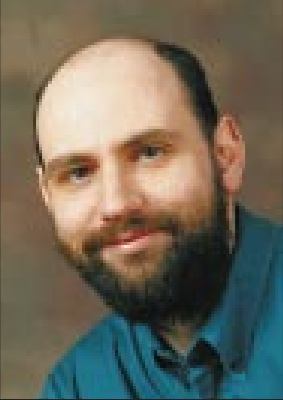
\includegraphics[width=0.22\textwidth]{fowler.png}
{\caption*{Martin Fowler, consultor independiente en Boston, Massachusetts. fowler@acm.org}}
\end{figure}

Hay muchas personas que creen que la adopción de UML es uno de los desarrollos más importantes en los últimos años. Pese a que estoy de acuerdo en que resolver conflictos menores sobre la notación es un gran paso, todavía tenemos un conjunto de preguntas más fundamentales: ¿Para qué sirve exactamente UML? ¿Por qué lo usamos? y, si no lo usamos, ¿por qué deberíamos? Si estás usando o pensando en usar UML deberías saber las respuestas a esas preguntas.

Es importante reconocer que crear un diagrama UML involucra un costo y un modelo UML no es algo que sea de fundamental importancia para un cliente. Los clientes quieren software que funcione, no imágenes, por más bonitas o estandarizadas que sean. Por lo tanto, el valor del modelado está enteramente ligado a su impacto en el software que estás produciendo. Si el modelo mejora la calidad o reduce el costo entonces el modelo tiene valor. Pero el modelo no tiene valor por sí mismo. Me recuerda al personaje de una novela (olvidada): \textquotedblleft Él era como el 0 en 90; con su esposa era algo, sin ella él no era nada\textquotedblright .

El valor que un modelo provee es fundamentalmente acerca de darle al usuario un entendimiento de algo que sea mayor que el software mismo. Esto puede ser un mayor entendimiento del software o del dominio que el software respalda. Lo puede hacer ya sea a través de una presentación gráfica bidimensional o resaltando información importante.

Un factor de complicación es que no todos los humanos piensan igual. Algunas personas entienden mejor las cosas en forma de texto; otras prefieren imágenes. Las personas difieren acerca de dónde están en esta escala y otras prefieren imágenes para algunos asuntos y texto para otros. Así que ten cuidado con los estándares excesivamente restrictivos. Recuerda que las necesidades individuales difieren y que necesitas encontrar cuál es la combinación más efectiva para la gente con la que estás trabajando.

Empezaré observando la simple transformación de texto a gráficos, dejando todos los detalles adentro. Con este enfoque tomas todo lo que puedes decir en texto y lo pones en el modelo. Esto toma mucho trabajo; hacer este nivel de detalle con el modelo y con el código fuente lleva demasiado tiempo para que valga la pena, a menos que tengas las herramientas que automaticen la tarea. Aquí es donde muchas herramientas CASE entran en juego: ya sea de ida y vuelta, en donde las herramientas convierten el modelo en código y al revés (por ejemplo, Rational Rose); o sin conversión, en donde el código es el mecanismo de almacenamiento para el modelo (por ejemplo, Together-J).

El costo de producir el modelo se reduce, aunque todavía hay un costo. Sin embargo, cuando tienes un modelo así de detallado debes preguntarte cuánto estás ganando. Creo que se puede ganar en relaciones estructurales (como estructuras de datos), pero a menudo se pierde claridad con flujo de control.

Otra función importante de los modelos es resaltar. Es difícil entender un sistema complejo al sumergirse en todos sus detalles. Puedes usar un modelo para resaltar solamente las partes importantes del sistema y lo puedes hacer antes de crear el software o después de que hayas construido el código. La cuestión es que puedas primero entender las estructuras claves que hacen que el software funcione y luego estarás en una mejor posición para investigar todos los detalles.

Nótese que digo \textquotedblleft resaltar los detalles importantes\textquotedblright{} y no \textquotedblleft ignorar los detalles\textquotedblright . Una visión de alto nivel que ignora todos los detalles suele carecer de valor porque no te dice nada. En lugar de una visión de alto nivel prefiero pensar en este estilo como un modelo esquelético. Te muestra los huesos del sistema, los cuales pueden ser bastante detallados.

En mi opinión un modelo esquelético es mejor que un modelo de cuerpo entero. Cuando estoy tratando de entender un modelo debo darme cuenta de dónde empezar. Típicamente las personas hacen esto tratando de encontrar las cosas importantes, pero dado que ellos no saben qué es lo importante, es mucho más fácil hacer que la persona que conoce el modelo haga la selección. Similarmente, si estoy creando un modelo antes de construir el sistema, las decisiones importantes están en esos detalles importantes. No todos los asuntos son igualmente importantes, y yo tengo un poder cerebral limitado. Necesito expandir ese poder en los detalles importantes, por lo que uso un modelo esquelético.

También me he dado cuenta de que un modelo esquelético es más fácil de mantener que uno de cuerpo entero. Los detalles importantes cambian con menos frecuencia. Y el modelo esquelético es más útil, por lo que las personas tienden a mantenerlo actualizado. Si la gente quisiera detalles, pueden explorar el código una vez que el esqueleto les haya provisto una visión general. Lo bueno del código es que siempre está en sintonía consigo mismo.

Lo esencial es que un modelo es o bien de cuerpo entero o esquelético, no puede ser ambas. O bien incluyes todos los detalles, o decides dejar algo afuera. Tan pronto como dejes algo afuera, estás yendo por el camino esquelético, incluso pese a que tu esqueleto pueda parecer menos anoréxico que el mío. Tu decisión estará basada en lo que encuentres más valioso para visualizar el sistema. La gente varía, por lo que tu decisión será diferente de la de otras personas, pero necesitas hacer una elección explícita.

Este es un problema clave con muchas herramientas CASE. La moda en estos días es que las herramientas CASE mantengan un vínculo automatizado con el código. Una herramienta, sin embargo, no puede diferenciar detalles importantes de asuntos secundarios, por lo que el resultado siempre es de cuerpo entero. Esto es empeorado por el hecho de que las herramientas típicamente basan su análisis en la estructura de datos de las clases en lugar de las interfaces. El principal objetivo de trabajar con objetos es que veas las interfaces, no la estructura de datos interna, así que el típico diagrama de ingeniería inversa te muestra exactamente las cosas que deberían estar ocultas. Los proveedores de herramientas CASE necesitan dedicarle más tiempo a pensar en cómo mostrarle al usuario cosas importantes y en cómo ocultar cosas que deberían permanecer en secreto. Por supuesto, como la definición de importante para todos es distinta, esto significa que hay mucha personalización complicada por hacer.

Por lo tanto, el dilema inevitable: para poder ver la madera de los árboles en el diseño, necesitas un modelo esquelético. Sin embargo, ni bien hagas esto, pierdes la habilidad de tener una conexión automatizada con los detalles.

No creo que vayamos a ver una solución de los proveedores CASE en el corto plazo. Si quieres un modelo que realmente comunique de manera efectiva, necesitas hacer un modelo esquelético, y eso significa que lo tienes que construir tú mismo. Al final es el cerebro humano el que cuenta.

Como nota final, quisiera agradecer a Derek Coleman por ayudarme a cristalizar mis pensamientos en esta columna con la asistencia de un buen vino y una servilleta de papel\textemdash dos de las herramientas de diseño más efectivas (y agradables) del mundo.

\end{document}
